
%%%%%%%%%%%%%%%%%%%%%%% file typeinst.tex %%%%%%%%%%%%%%%%%%%%%%%%%
%
% This is the LaTeX source for the instructions to authors using
% the LaTeX document class 'llncs.cls' for contributions to
% the Lecture Notes in Computer Sciences series.
% http://www.springer.com/lncs       Springer Heidelberg 2006/05/04
%
% It may be used as a template for your own input - copy it
% to a new file with a new name and use it as the basis
% for your article.
%
% NB: the document class 'llncs' has its own and detailed documentation, see
% ftp://ftp.springer.de/data/pubftp/pub/tex/latex/llncs/latex2e/llncsdoc.pdf
%
%%%%%%%%%%%%%%%%%%%%%%%%%%%%%%%%%%%%%%%%%%%%%%%%%%%%%%%%%%%%%%%%%%%


\documentclass[runningheads,a4paper]{llncs}

\usepackage{amssymb}
\setcounter{tocdepth}{3}
\usepackage{graphicx}

\usepackage{url}
\urldef{\mailsa}\path|{alfred.hofmann, ursula.barth, ingrid.haas, frank.holzwarth,|
\urldef{\mailsb}\path|anna.kramer, leonie.kunz, christine.reiss, nicole.sator,|
\urldef{\mailsc}\path|erika.siebert-cole, peter.strasser, lncs}@springer.com|    
\newcommand{\keywords}[1]{\par\addvspace\baselineskip
\noindent\keywordname\enspace\ignorespaces#1}

\begin{document}

\mainmatter  % start of an individual contribution

% first the title is needed
\title{Lecture Notes in Computer Science:\\Authors' Instructions
for the Preparation\\of Camera-Ready
Contributions\\to LNCS/LNAI/LNBI Proceedings}

% a short form should be given in case it is too long for the running head
\titlerunning{Lecture Notes in Computer Science: Authors' Instructions}

% the name(s) of the author(s) follow(s) next
%
% NB: Chinese authors should write their first names(s) in front of
% their surnames. This ensures that the names appear correctly in
% the running heads and the author index.
%
\author{Alfred Hofmann}%

%
\authorrunning{Lecture Notes in Computer Science: Authors' Instructions}
% (feature abused for this document to repeat the title also on left hand pages)

% the affiliations are given next; don't give your e-mail address
% unless you accept that it will be published
\institute{Springer-Verlag, Computer Science Editorial,\\
Tiergartenstr. 17, 69121 Heidelberg, Germany\\
\mailsa\\
\mailsb\\
\mailsc\\
\url{http://www.springer.com/lncs}}

%
% NB: a more complex sample for affiliations and the mapping to the
% corresponding authors can be found in the file "llncs.dem"
% (search for the string "\mainmatter" where a contribution starts).
% "llncs.dem" accompanies the document class "llncs.cls".
%

\toctitle{Lecture Notes in Computer Science}
\tocauthor{Authors' Instructions}
\maketitle


\begin{abstract}
The abstract should summarize the contents of the paper and should
contain at least 70 and at most 150 words. It should be written using the
\emph{abstract} environment.
\keywords{We would like to encourage you to list your keywords within
the abstract section}
\end{abstract}


\section{Introduction}
Social media has greatly democratized content creation. Facebook, Twitter, Skype, Whatsapp and LiveJournal are commonly used to share any thoughts and opinions about anything in the surrounding world. All this content has created new opportunities to study public opinion. Twitter is especially popular for research due to its scale, representative, variety of topics discussed and its ease access to content. In the past years, research in that direction was hindered by the unavailability of suitable datasets and lexicons for system training, development and testing. Some Twitter-specific resources were developed, but they were either small and proprietary, or they relied on noisy labels obtained automatically. This all changed with the shared task on Sentiment Analysis on Twitter, which is part of the international Worksop on Semantic Evaluation. The task is active since 2013 and it attract over 40+ participant teams. It contains 5 subtasks with their train and test datasets. First task is Message Polarity Classification, where we need to classify whether the given message is of positive, negative, or neutral sentiment. In second and third task, there is beside a given message, also a topic and you need to classify the message on two point scale and five-point scale, depending on the task. Forth and fifth task are also on two point and five point scale, where there are given tweets about a given topic, and you need to estimate their distribution.



\section{Dataset}
For tasks we are provided with their datasets with annotated tweets. They are gathered in a way, that express sentiment about popular topics. For this purpose, they extracted named entities from millions of tweets. The collected tweets were greatly skewed towards the neutral class. To reduce the class imbalance, they removed those that contained no sentiment-bearing words. Tweets are then manually filtered to obtain a set of meaningful topics with at least 100 tweets each. Topics that are ambiguous (e.q.., Barcelona, which is a city or sport club) or too general (e.q., Paris). The topics in the training and in the test data do not overlap, meaning that test tweets consist of topics that are different from the topics in train dataset. Dataset is consisted of four parts: TRAIN (for training models), DEV (for tuning models), DEVTEST (for development-time evaluation) and TEST (for official evaluation). The first three datasets were annotated using Amazon's Mechanical Turk , while the TEST dataset was annotated on CrowdFlower. 

\section{Related work}
There are a lot of related work, that also competed in Sentiment Analysis in Twitter.

 In work~\cite{vilaresa2016lys}, they have trained convolutional neural network (CNN) to extract hidden activation values from the hidden layers once some input had been fed to the network. That values served as features for SVM model. They have discovered that CNN serves good as feature extractor but not as good as independent classifier. They have received good results and were on the top of the rankings list. Their best results were for tasks B (2./14),C(4/11) and D(2/14). Their approach is very different from ours since they entirely use models with machine learning and our method is more calculating similarities between tweets. 

In work~\cite{briones2016vcu} they have used simple unigram model baseline with three main features enchantments incorporated into the model. This features are emoticon retention, word stemming and token saliency calculation. This work is similar to ours, since they also uses TF-IDF to calculate similarities between tweets. They preprocessed text with word stemming, while we used lemmatizing. With stemming or lemmatizing, the emoticons get lost. In order to preserve emoticons, they have extracted it before stemming and use them as features. They also used unigrams to achieve better results. We didn't used them because we got worst performance.

\subsection{Evaluation and discussion}


\subsection{Subtask A: Message polarity classification}
Subtask A is a single-label multi-class(SLMC) classification task. Each tweet must be classified as positive, neutral or negative. The evaluation score is measured as $F^{PN}_1$:
\begin{equation}
F^{PN}_1 = \frac{F^P_1 + F^N_1}{2}
\end{equation}
$F_1^P$ is $F_1$ for the positive class:

\begin{equation}
F^{P}_1 = \frac{2\pi^P\varphi^P}{\pi^P + \varphi^P}
\end{equation}

Here $\pi^P$ and $\varphi^P$ denote precision and recall for the positive class, respectively: 

\begin{equation}
\pi^P = \frac{PP}{PP + PU + PN}
\end{equation}

\begin{equation}
\varphi^P = \frac{PP}{PP + UP + NP}
\end{equation}

where $PP$, $UP$, $NP$, $PU$, $PN$ are the cells of the confusion matrix shown in table. 

\begin{center}
  \begin{tabular}{ | l | l | c | r |}
    \hline
  predicted/real   & positive & neutral & negative \\ \hline
   positive  & PP & PU & PN \\ \hline
   neutral  & UP & UU & UN \\ \hline
   negative  & NP & NU & NN \\
    \hline
  \end{tabular}
\end{center}

\subsection{Subtask B: Tweet classification according to a two-point scale}
For subtask B each tweet must be classified as either positive or negative. For this subtask they have adopted macro-averaged recall: 

\begin{equation}
\varphi^{PN} = \frac{1}{2}(\varphi^P + \varphi^N) \\
= \frac{1}{2}(\frac{PP}{PP + NP} + \frac{NN}{NN + PN})
\end{equation}
$\varphi^{PN}$ ranges from 0 to 1, where a value of 1 is the best score, while 0 means that classifier misclassified all items. This method is better than classic accuracy because its more robust to class invariance. 

The evaluation for subtask B is evaluated independently for each topic. The results are then averaged across topics to yield the final score.


\subsection{Subtask C: Tweet classification according to a five-point scale}

Subtask is an ordinal classification task, in witch each tweet must be classified into exactly one of the classes that are highly-positive, positive, neutral, negative and highly-negative. Classes are represented as numbers {+2, +1, 0, -1, -2} in mentioned above order. For evaluation we use macro-averaged mean absolute error ($MAE^M$):

\begin{equation}
MAE^M(h, Te) = \frac{1}{|C|}\sum_{j=1}^{|C|}\frac{1}{|Te_j|}\sum_{x_i\in Te_j}|h(x_i) - y_i|
\end{equation}
where $y_i$ denotes the true label of item $x_i$ and $h(x_i)$ is its predicted value. $Te_j$ denotes the set of test document whose true class is $c_j$ and $|h(x_i) - y_i|$ denotes the distance between classes $h(x_i)$ and $y_i$. The advantage of $MAE^M$ over standard $MAE$ is that it is robust to class imbalance. Unlike the previous mentioned methods, the lower the score value is, the better results are. 



\subsection{Subtask D: Tweet quantification according to a two point scale}

Subtask D assumes a binary quantification setup, in which each tweet is classified as positive or negative. The task is to compute an estimate of the distribution of each of the classes. For evaluation there is used normalized cross-entropy, known as Kullback-Leibler Divergence ($KLD$):

\begin{equation}
KLD(q, p, C) = \sum_{c_j \in C}p(c_j)\log_e\frac{p(c_j)}{q(c_j)}
\end{equation}
$KLD$ is a measure of the error made in estimating a true distribution $p$ over set of classes ($C$) by means of a predicted distribution $q$. $KLD$ ranges between 0 and $+\inf$, where lower value is better. $KLD$ is computed individually for each topic, and results are averaged to yield the final score.

\subsection{Subtask E: Tweet quantification according to a five-point scale}

Subtask E is an ordinal quantification (OQ) task, in which each tweet belongs exactly to one of the classes : highly positive, positive, neutral, negative, highly negative. The measure used for OQ is the Earth Mover's Distance ($EMD$):  

\begin{equation}
EMD(q, p) = \sum_{j=1}^{|C| - 1}|\sum_{i=1}^jq(c_i) - \sum_{i=1}^jp(c_i)|
\end{equation}

This is also a measure of error, therefore lower values are better.$EMD$ is computed individually for each topic, and results are then averaged across all topics to yield the final score.
\begin{figure}
\centering
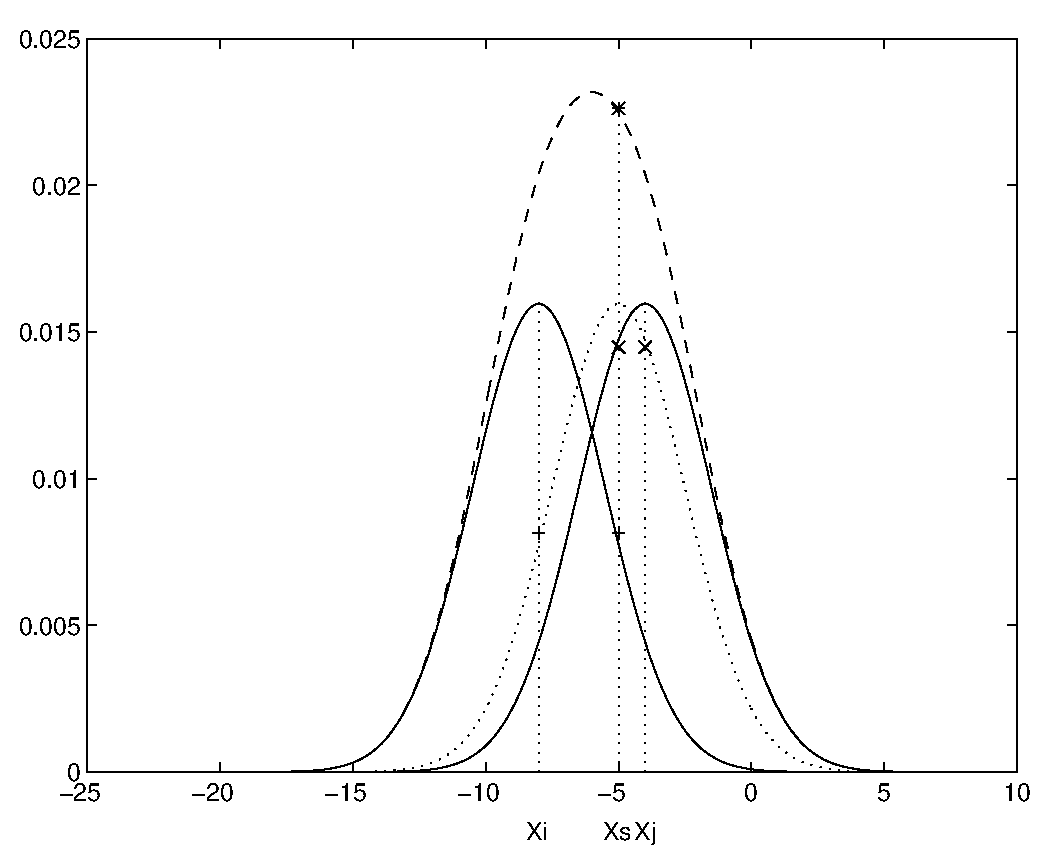
\includegraphics[height=6.2cm]{eijkel2}
\caption{}
\label{fig:example}
\end{figure}









\begin{thebibliography}{4}

\bibitem{jour} Smith, T.F., Waterman, M.S.: Identification of Common Molecular
Subsequences. J. Mol. Biol. 147, 195--197 (1981)

\bibitem{lncschap} May, P., Ehrlich, H.C., Steinke, T.: ZIB Structure Prediction Pipeline:
Composing a Complex Biological Workflow through Web Services. In: Nagel,
W.E., Walter, W.V., Lehner, W. (eds.) Euro-Par 2006. LNCS, vol. 4128,
pp. 1148--1158. Springer, Heidelberg (2006)

\bibitem{book} Foster, I., Kesselman, C.: The Grid: Blueprint for a New Computing
Infrastructure. Morgan Kaufmann, San Francisco (1999)

\bibitem{proceeding1} Czajkowski, K., Fitzgerald, S., Foster, I., Kesselman, C.: Grid
Information Services for Distributed Resource Sharing. In: 10th IEEE
International Symposium on High Performance Distributed Computing, pp.
181--184. IEEE Press, New York (2001)

\bibitem{proceeding2} Foster, I., Kesselman, C., Nick, J., Tuecke, S.: The Physiology of the
Grid: an Open Grid Services Architecture for Distributed Systems
Integration. Technical report, Global Grid Forum (2002)

\bibitem{url} National Center for Biotechnology Information, \url{http://www.ncbi.nlm.nih.gov}

\end{thebibliography}

@inproceedings{vilaresa2016lys,
  title={LYS at SemEval-2016 Task 4: Exploiting neural activation values for Twitter sentiment classification and quantification},
  author={Vilaresa, David and Dovala, Yerai and Alonsoa, Miguel A and G{\'o}mez-Rodr{\i}gueza, Carlos},
  booktitle={Proceedings of the 10th International Workshop on Semantic Evaluation (SemEval 2016), San Diego, US},
  year={2016}
}

@article{briones2016vcu,
  title={VCU-TSA at Semeval-2016 Task 4: Sentiment Analysis in Twitter},
  author={Briones, Gerard and Amarasinghe, Kasun and McInnes, Bridget T},
  journal={Proceedings of SemEval},
  pages={215--219},
  year={2016}
}

\end{document}
